%==============================================================================
\section{Results for the Baseline Geometry}
\label{sec:results_baseline}
%==============================================================================

\begin{table}[htpb]
 \caption{Uncertainties on all systematic parameters for the baseline
  detector model with three years of lifetime, ranked according to their impact
  on the mass hierarchy parameter $h$.}
 \label{tab:baseline_results}
 \begin{center}
  \small{\begin{tabular}{lrrrrrr} 
\toprule
Parameter & Impact [\%] & Best Fit & $\sigma^\mathrm{full}$ & $\sigma^\mathrm{stat}$ & $\sigma^\mathrm{syst}$ & Prior \\ 
\midrule
$h$ & 100.0 & \num{1.00e+00} & \num{3.43e-01} & \num{2.33e-01} & \num{2.52e-01} & free \\
$r_{A_\mathrm{eff},\,\nu-\bar\nu}$ & 8.9 & \num{0.00e+00} & \num{4.73e-02} & \num{4.76e-03} & \num{1.47e-01} & \num{5.00e-02} \\
$\vartheta_{13}$ [$^\circ$] & 8.0 & \num{8.93e+00} & \num{4.64e-01} & \num{8.24e-01} & \num{3.67e+00} & \num{4.68e-01} \\
$n_{A_\mathrm{eff}}$ & 7.4 & \num{0.00e+00} & \num{1.94e-02} & \num{1.99e-03} & \num{1.94e-02} & \num{2.00e-01} \\
$\vartheta_{23}$ [$^\circ$] & 3.2 & \num{3.86e+01} & \num{4.67e-01} & \num{3.02e-01} & \num{3.97e-01} & \num{1.32e+00} \\
$\Delta m^2_{31}$ [eV$^2$] & 2.7 & \num{2.46e-03} & \num{6.49e-05} & \num{1.77e-05} & \num{1.10e-04} & \num{8.00e-05} \\
$r_{\Phi,\,\nu_e-\nu_\mu}$ & 2.4 & \num{0.00e+00} & \num{1.10e-02} & \num{5.12e-03} & \num{1.01e-02} & \num{5.00e-02} \\
$s_{A_\mathrm{eff}}$ [m$^2$/GeV] & 1.1 & \num{0.00e+00} & \num{2.19e-04} & \num{1.23e-04} & \num{1.82e-04} & free \\
$\Delta_\mathrm{PID}$ [GeV] & 0.9 & \num{0.00e+00} & \num{1.70e-02} & \num{1.58e-02} & \num{6.23e-03} & \num{5.00e-01} \\
$s_E$ & 0.1 & \num{1.00e+00} & \num{2.81e-02} & \num{7.66e-03} & \num{3.31e-02} & \num{5.00e-02} \\
\bottomrule 
\end{tabular}
}
 \end{center}
\end{table}

\noindent
Using the settings described in the previous section, the Fisher matrix for
PINGU can now be constructed with \papa. The full, statistical, and systematic
errors are for all parameters are listed in Tab.~\ref{tab:baseline_results} for
a nominal PINGU lifetime of three years. The parameters are ordered after their
\emph{impact} on the mass hierarchy parameter $h$, which is defined as the
square of their correlation coefficient $c_{ih}$ (\ref{eqn:corr_coeff}) with
$h$. Note that for the baseline settings, the systematic parameter
$s_\mathrm{PID}$ has been excluded as it is fully degenerate with $n_{\aeff}$:
since the PID decision is binary, no channel of unidentified events exists and
hence both parameters just evenly increase the overall number of events,
effectively.

From the first line of Tab.~\ref{tab:baseline_results}, one can read off the
expected significance of PINGU's mass hierarchy measurement by inverting the
full error (see Sec.~\ref{sec:fisher_hierarchy}). This gives an expected
significance of 2.9\,$\sigma$ after three years. Looking at the statistical
error alone, the significance increases to 4.3\,$\sigma$, emphasising the 
important role systematic parameters are playing in the determination of the 
mass hierarchy.

\begin{figure}[bhtp]
 \centering
 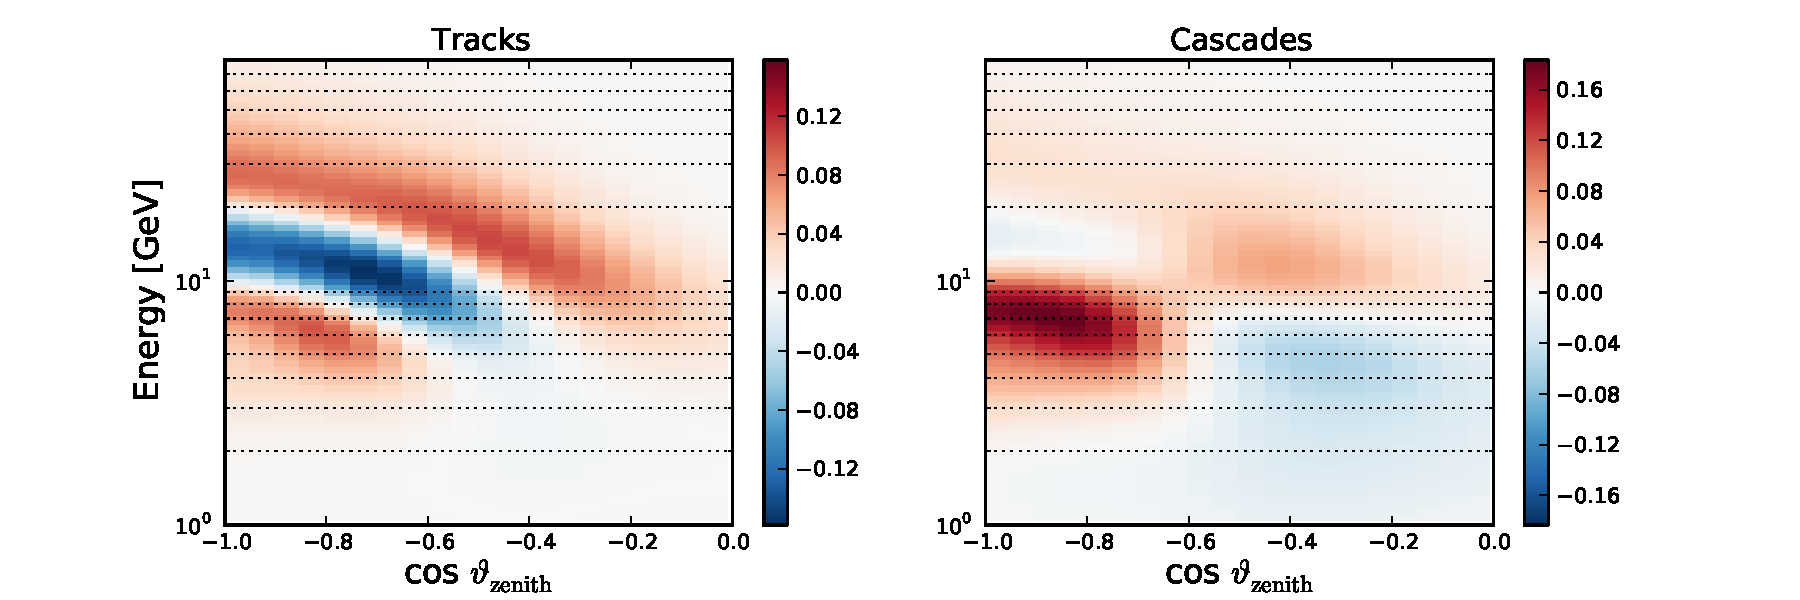
\includegraphics[width=\linewidth]{akhmedov_baseline}
 \caption{\delchi distribution in the track (left) and cascade (right) channels 
for the baseline settings.}
 \label{fig:akhmedov_baseline}
\end{figure}

\begin{figure}[thp]
 \centering
  \subfloat[\label{fig:sigma_vs_time}]
   {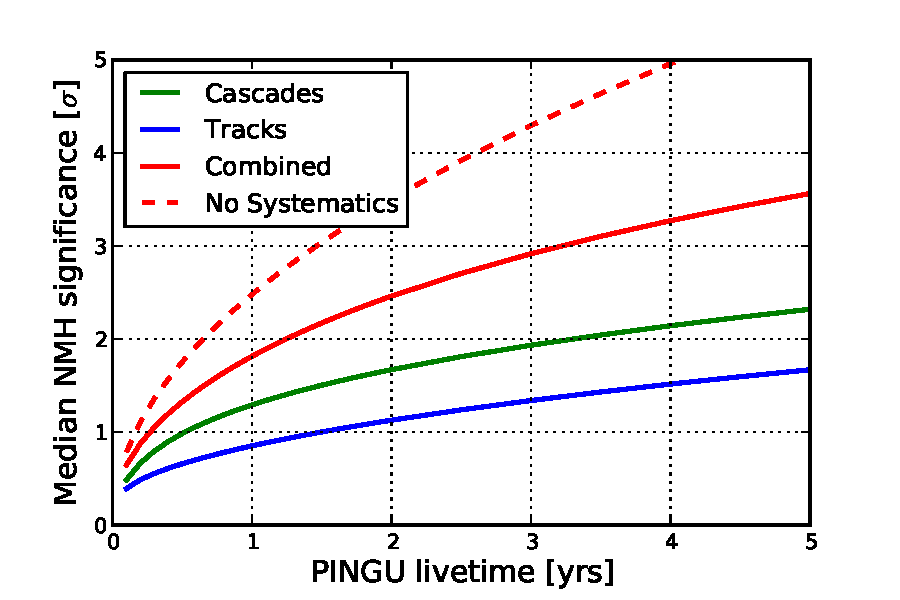
\includegraphics[width=0.495\linewidth]{sigma_vs_time_default}}
  \subfloat[\label{fig:covmat_baseline}] 
   {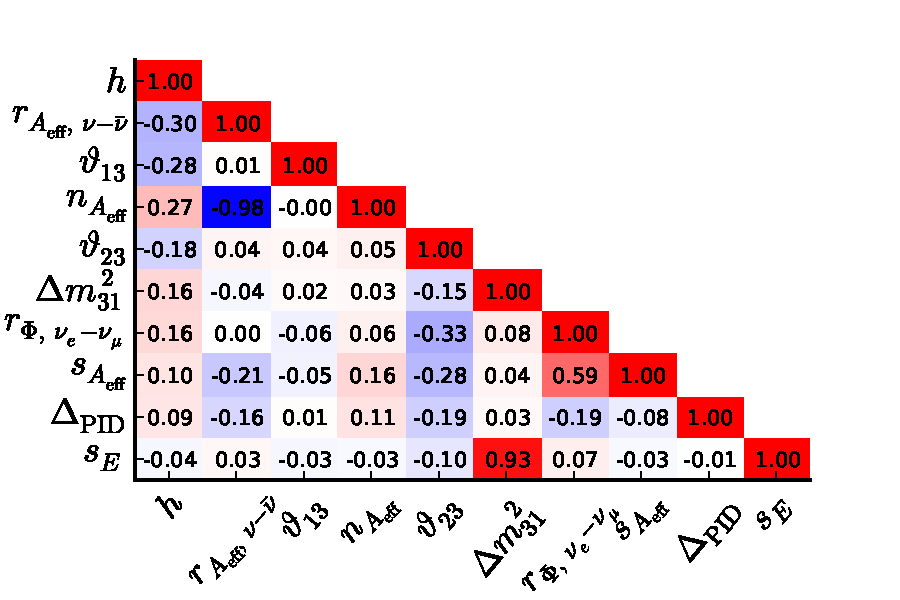
\includegraphics[width=0.495\linewidth]{CovMat_PINGU}}
 \caption{\protect\subref{fig:sigma_vs_time} Evolution of PINGU's expected mass 
          hierarchy significance with time and 
          \protect\subref{fig:covmat_baseline} full correlation matrix for PINGU
          for the baseline settings.}
 \label{fig:time_covmat}
\end{figure}

Treating the track and cascade channels separately, the expected significances
are 1.9\,$\sigma$ with and 3.0\,$\sigma$ without systematics for the cascade
and 1.3\,$\sigma$ (3.1\,$\sigma$) for the track channel,
respectively\footnote{The full error listings corresponding to
Tab.~\ref{tab:baseline_results} can be found in
App.~\ref{app:fisher_baseline}}. Although the purely statistical significances
are comparable, when taking systematics into account the significance for the
cascades remains much higher than the track significance. 
The reason for this becomes obvious when looking at the \delchi distributions 
for both channels in Fig.~\ref{fig:akhmedov_baseline}. In the track channel, 
there are three distinct regions driving the expected significance. These 
regions are separated only by small margins and have alternating sign, while in 
the cascade channel most of the significance comes from one contiguous region. 
Together with the fact that the cascade channel has roughly three times higher 
event statistics than the track channel---62,000 vs.\ 22,000 neutrino events 
per year---this makes the cascade channel much more robust against the impact 
of systematic parameters.

In Fig.~\ref{fig:sigma_vs_time}, the significances for the individual channels 
and for their combination are shown as a function of time. The purely 
statistical significance is plotted as well, exhibiting a scaling with the 
square root of the lifetime as one would expect for a counting experiment where 
the relative error is proportional to $1/\sqrt{N}$. The actual significances 
including systematics increase much slower with time as a part of the 
accumulating statistics has to be ``spent'' in order to better constrain the 
systematic parameters. However the combined analysis of the two channels still 
gives a much higher sensitivity than simply adding the two individual channels 
in quadrature as one would do for two completely unrelated measurements of the 
same quantity. E.\,g.\ for a lifetime of three years as above, the quadratic 
sum of the track and cascade significances is $\sqrt{(1.3\,\sigma)^2 + 
(1.9\,\sigma)^2} \approx 2.3\,\sigma$, considerably lower than the 
2.9\,$\sigma$ for the combined analysis.

Finally one can look at the correlation matrix of PINGU. In contrast to the 
error listing for all parameters as in Tab.~\ref{tab:baseline_results}, here the 
interdependences between the parameters are in the focus. The graphical 
representation in Fig.~\ref{fig:covmat_baseline} shows, for every combination 
of parameters, their correlation coefficient $c_{ij}$. Using these quantities 
instead of the entries $\sigma_{ij}$ of the covariance matrix themselves has 
the benefit that due to their normalisation, cf.~(\ref{eqn:corr_coeff}), the 
entries of the matrix are dimensionless and restricted to the range $[-1, +1]$, 
thus making them easier to interpret.

From the correlation matrix itself, several things can be learned. First, the 
hierarchy parameter is the one with strongest overall correlations. This 
emphasises the fact that the determination of the neutrino mass hierarchy is a 
very delicate measurement relying on a small effect, and that the inclusion of 
so many systematic parameters is indeed necessary to get a robust result.

\begin{figure}[thp]
 \centering
 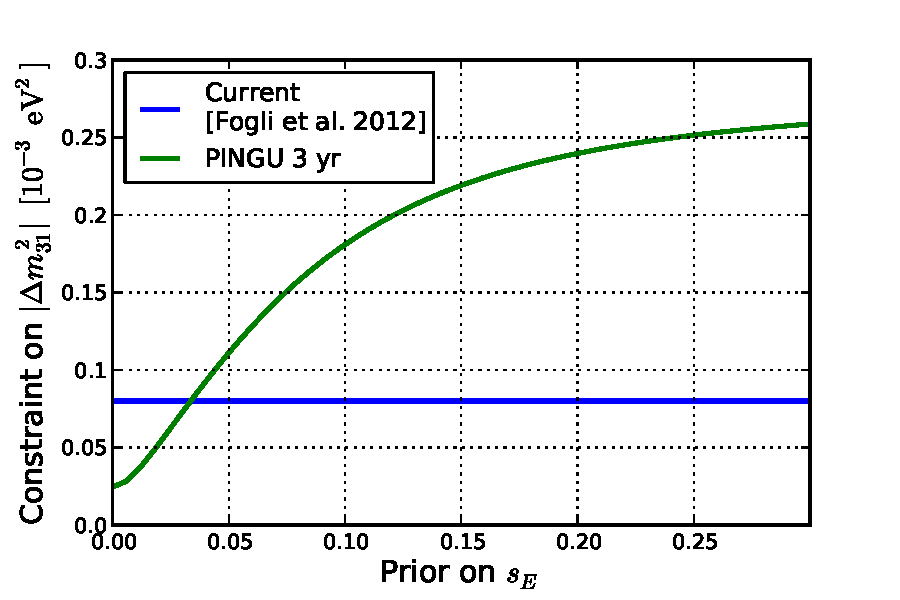
\includegraphics[width=0.7\linewidth]{dm31_vs_escale_prior}
 \caption{PINGU constraint on \dm{31} as a function of the prior on the energy
          scale. No prior knowledge about \dm{31} is assumed.}
 \label{fig:dm31_vs_escale_prior}
\end{figure}

Furthermore, two combinations of parameters stick out due to their very strong 
correlation. The first one is the relative normalisation of the effective areas 
for neutrinos and antineutrinos, $r_{\aeff,\,\nu-\bar\nu}$, and the overall 
normalisation 
of all effective areas, $n_{\aeff}$. Their anticorrelation is obvious from 
their definition: $r_{\aeff,\,\nu-\bar\nu}$ increases the number of neutrino 
events while decreasing the number of antineutrino events. Since PINGU cannot 
distinguish between those and the cross-section for neutrinos is higher 
approximately by a factor of two (see Fig.~\ref{fig:NuXsec_GeV}), the total 
number of events is increased, which can be compensated by decreasing 
$n_\aeff$. Only the MSW resonance oscillation causes an asymmetry between 
neutrinos and antineutrinos, such that the anticorrelation is not exactly $-1$.

The second strong correlation can be observed between the absolute value of the 
mass splitting \dm{31} and the energy scale $s_E$. The value of \dm{31} is 
determined from the position of the oscillation minimum in the track channel 
that is easy to spot in Fig.~\ref{fig:SimSteps}. In a two-flavour approximation, 
this can be described by equation (\ref{eqn:osc_length}), where the oscillation 
length is determined by the zenith angle. Then the size of \dm{31} is inversely 
proportional to the neutrino energy at which the oscillation minimum appears. 
Thus a larger value of \dm{31} can be compensated by increasing the energy scale 
accordingly.

This means that if PINGU is supposed to make a precise measurement of \dm{31}, 
the energy scale has to be known very accurately. As the energy of a neutrino 
event is determined primarily from the number of detected photons\footnote{The 
Cherenkov light output is directly proportional to the deposited energy.}, this
means that the photon detection efficiency of the optical modules has to be
well calibrated. This behaviour is illustrated in
Fig.~\ref{fig:dm31_vs_escale_prior}, where PINGU's self-contained constraint on
the value of \dm{31} is plotted against the prior put on $s_E$. To improve on
the current limits, the energy scale has to be known with an accuracy of at
least 3\,\%.

\subsection{Measuring the Atmospheric Mixing Parameters}
\label{sec:results_atmosperic}

\begin{figure}[thp]
 \centering
 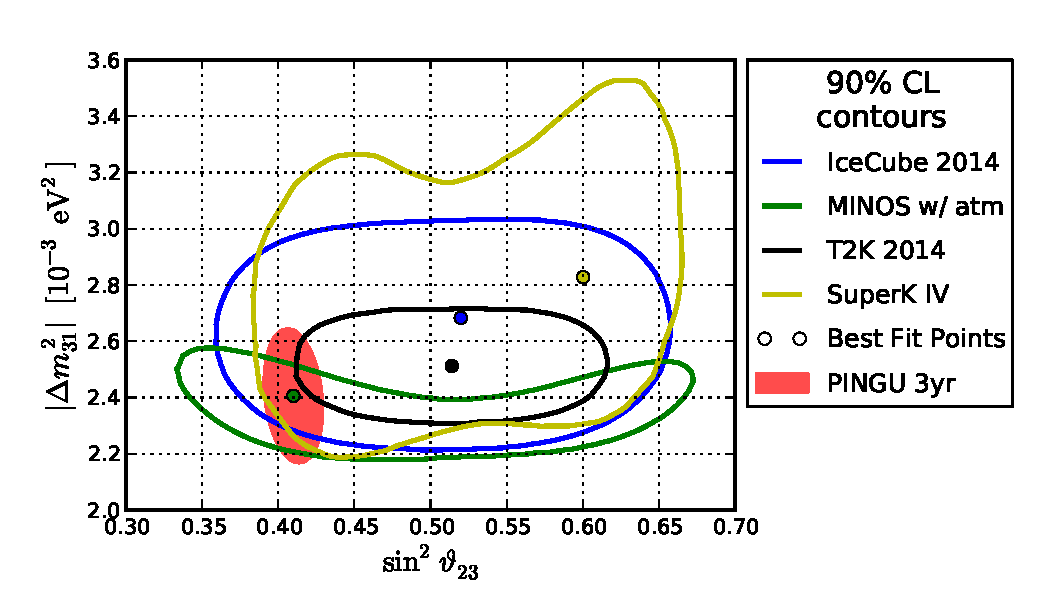
\includegraphics[width=0.85\linewidth]{AtmoParamsBaseline}
 \caption{PINGU constraint on \dm{31} and $\sin^2\thet{23}$ for the baseline
          settings. No prior knowledge about the two parameters is assumed.
          The latest constraints from the IceCube/DeepCore \cite{DCosc}, MINOS
          \cite{MINOSparams}, T2K \cite{T2Kparams}, and SuperKamiokande
          \cite{SuperKparams} are shown for reference.}
 \label{fig:AtmoParamsBaseline}
\end{figure}

To determine the neutrino mass hierarchy, PINGU makes a precision measurement
of the oscillations of atmospheric neutrinos. In fact, with more than 80,000
events recorded per year it will collect the largest sample of atmospheric
neutrinos so far. After DeepCore has been established as a serious contributor
to the global effort of characterising neutrino oscillations, PINGU will go
even further into that direction and provide tight constraints on the values of
\dm{31} and in particular \thet{23}.

\begin{figure}[tbhp]
 \centering
 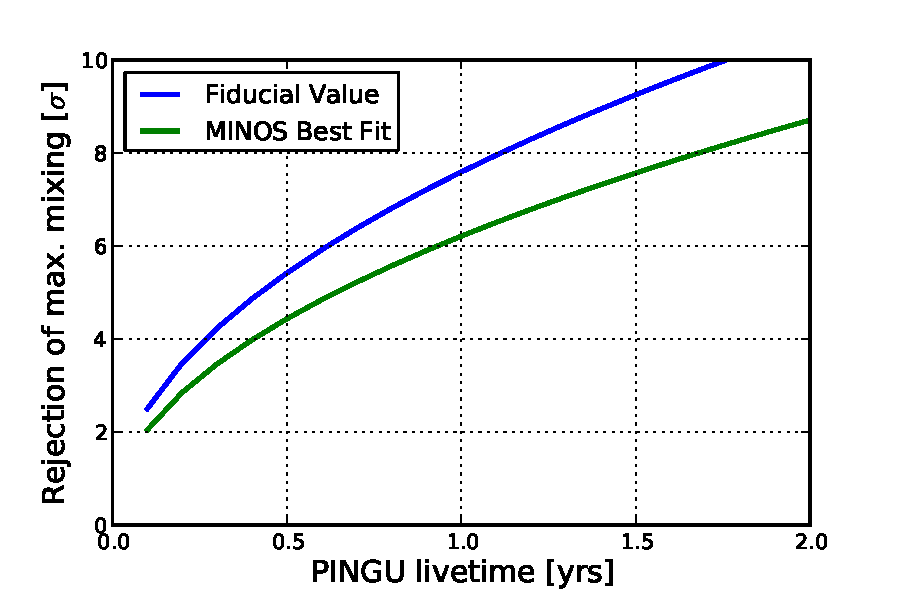
\includegraphics[width=0.7\linewidth]{Exclude_MaxMix}
 \caption{Confidence level of rejecting the maximal mixing case as a function
  of PINGU's lifetime for different true values of \thet{23}.}
 \label{fig:Exclude_MaxMix}
\end{figure}

These constraints are shown in Fig.~\ref{fig:AtmoParamsBaseline}, along with
the most recent confidence regions of current oscillation experiments. For
PINGU, no priors have been put on \dm{31} or \thet{23}, meaning that the
displayed confidence ellipse comes from PINGU data alone and does not profit
from external knowledge.

The most obvious feature of PINGU's confidence ellipse is its orientation,
which is different from the other experiments: While it cannot constrain
\dm{31} any better than current experiments, the value of \thet{23} will be
much more precise than any measurement available today. The reason for this is
that the value of \dm{31} is extracted from the position of the oscillation
minimum in energy, which needs a precise calibration of the energy scale as 
shown above. This is much easier to achieve in experiments on a neutrino
beam like MINOS or T2K where the beam energy is well-known. \thet{23} on the
other hand is determined from the relative depth of the oscillation minimum as
one can see from equation (\ref{eqn:twoflavour_prob}). Here PINGU profits from
its wide energy range including control regions without oscillations and the
large event statistics, such that especially the overall detector
efficiency\footnote{Represented by $n_\aeff$ in \papa.}, which usually is
difficult to constrain in beam experiments, only has minor impact.

From the error contours in Fig.~\ref{fig:AtmoParamsBaseline} one can also see
that the value of the mixing angle \thet{23} is not very tightly constrained
yet. So far, all experiments' results are compatible with the maximal mixing
value of $\thet{23}=45^\circ$\footnote{Since the ``strength'' of the mixing is
proportional to $\sin^2 2\theta$, see (\ref{eqn:twoflavour_prob}), it becomes
maximal for $\theta=45^\circ$.}, however MINOS's and SuperKamiokande's best
fit points are rather distant from maximal mixing.

Since PINGU will make a much more precise measurement of \thet{23} than any
current experiment, it will likely be able to exclude the maximal mixing case
with high confidence if the true value of \thet{23} is sufficiently offset from
$45^\circ$. In Fig.~\ref{fig:Exclude_MaxMix} the confidence which PINGU can
reject the maximal mixing hypothesis with is shown as a function of the
experimental lifetime. Although this depends on the assumed true value of
\thet{23}, it is obvious that PINGU is likely to exclude maximal mixing at the
5\,$\sigma$ level already after the first year of data taking.

\subsection{Impact of the Octant of \thet{23}}
\label{sec:results_octant}

As shown in the previous section, currently it is still unclear whether
\thet{23} is
smaller or larger than $45^\circ$. The fiducial value chosen for the baseline
analysis was the best fit point from the Fogli global fit \cite{Fogli}, which is
close to the MINOS best fit point and such gives a comparably small mixing
angle. 

Thus it is important to test whether the fiducial value of \thet{23} that is
chosen in \papa has any impact on the expected sensitivity to the mass
hierarchy. The \texttt{PhysicsSimulation} step, \ie the calculation of the
oscillation probabilities, has been repeated for several different fiducial 
values of \thet{23}, all larger than the baseline one. The resulting
oscillation probabilities were consecutively
processed through the \texttt{DetectorSimulation}. For each of these settings,
the sensitivity to the neutrino mass hierarchy has been evaluated for a
lifetime of three years and plotted against the injected fiducial value for
\thet{23} in Fig.\ref{fig:sigma_vs_th23}.

As it turns out, the sensitivity increases considerably as \thet{23} takes
larger values and even exceeds 5\,$\sigma$ in the second octant, \ie at values
above $45^\circ$. This increase in sensitivity comes exclusively from the
cascade channel, which already points to its origin: the oscillation of \numu
to \nue, which is mainly defined by this mixing angle. However the neutrinos
propagate through the Earth, so this angle has to be replaced by the
corresponding effective mixing angle in matter (\ref{eqn:matter_angle}), which
is further from maximal mixing than the vacuum value.

\begin{figure}[thp]
 \centering
  \subfloat[\label{fig:sigma_vs_th23}]
  {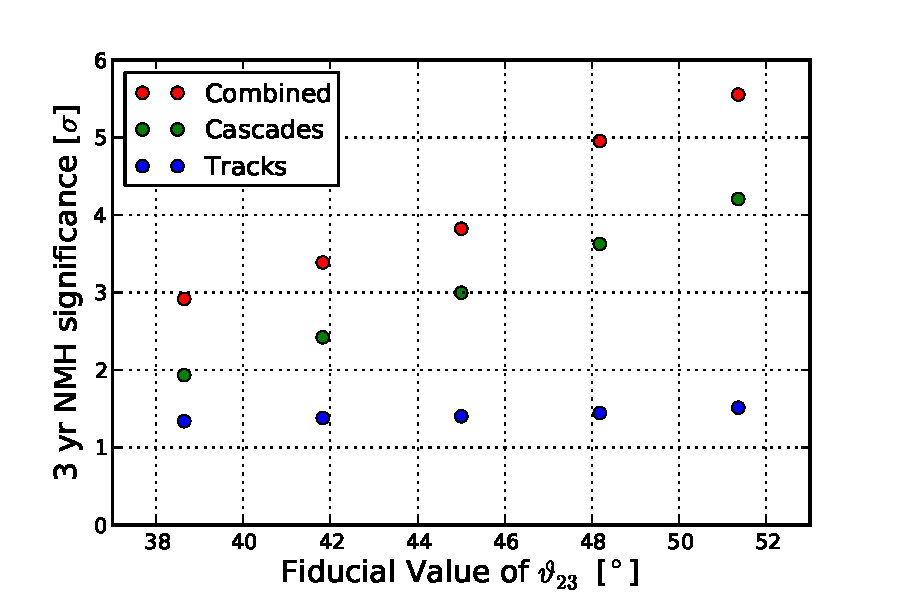
\includegraphics[width=0.495\linewidth]{sigma_vs_th23}}
  \subfloat[\label{fig:th_mat_vs_th23}]
  {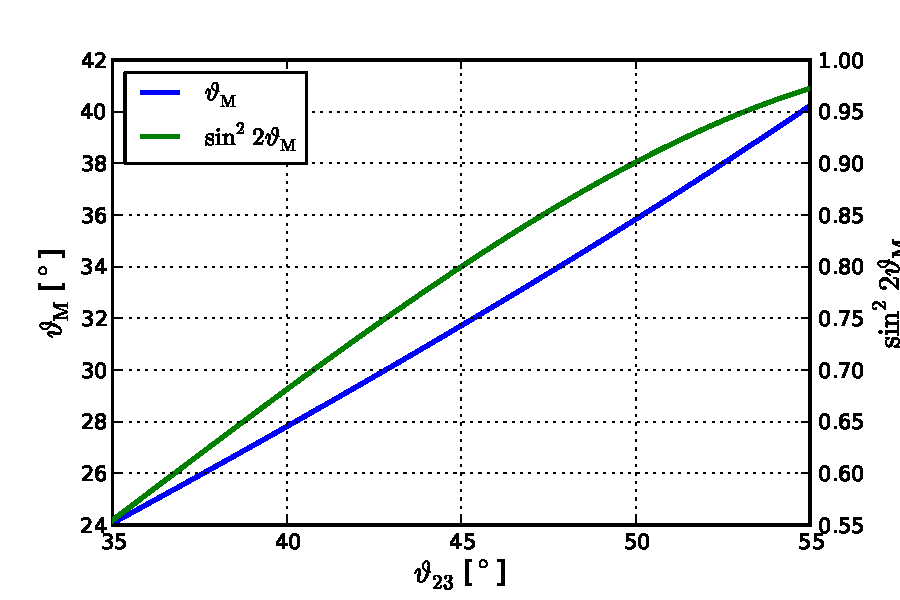
\includegraphics[width=0.495\linewidth]{th_mat_vs_th23}}
 \caption{PINGU three-year sensitivity to the neutrino mass hierarchy (a)
          and effective mixing angle in matter for $A_\mathrm{CC}/\dm{} = -0.5$
          (b) as a function of the fiducial value of \thet{23}.}
 \label{fig:scan_th23}
\end{figure}

The relation between matter and vacuum value of \thet{23} is shown
qualitatively in Fig.~\ref{fig:th_mat_vs_th23}. The choice of
$A_\mathrm{CC}/\dm{} = -0.5$ corresponds to a neutrino energy of $\approx
3.2$\,GeV at a matter density of 5\,g/cm$^{-3}$, the negative sign is due to 
$A_\mathrm{CC}$ being below zero as it caused by electrons with negative
charge, see (\ref{eqn:mat_pot}). So due to the effective reduction of \thet{23}
in matter,
the amplitude of the oscillation, proportional to $\sinsq{2\thet{\mathrm{M}}}$,
keeps growing even beyond $\thet{23}=45^\circ$, where for oscillations in
vacuum the amplitude would decrease again.
Consequently, increasing the overall scale of $\numu\to\nue$ oscillations
results in an increased absolute difference between the cascade event histograms
for normal and inverted mass hierarchy and hence a better sensitivity for the
hierarchy determination.

A beneficial side effect of the effective reduction of \thet{23} in matter is
that it causes the relation of the parameter, \thet{23}, and the observable,
the oscillation probability proportional to $\sinsq{2\thet{\mathrm{M}}}$, to be
in the linear regime, as shown in Fig.~\ref{fig:th_mat_vs_th23} as well. This
makes the evaluation in the Fisher matrix formalism well justified (cf.\
Sec.~\ref{sec:fisher_prereq}), whereas for vacuum oscillations the oscillation
probability $\sinsq{2\thet{23}}$ becomes an increasingly non-linear function
close to the maximal mixing value of \thet{23}.

In addition, the symmetry between values of \thet{23} in the first and second
octant, mirrored at $45^\circ$, gets broken. This symmetry can be found in
most of the confidence contours in Fig.~\ref{fig:AtmoParamsBaseline} and
affects all experiments that observe vacuum oscillations, making it difficult
to determine the actual octant of \thet{23} even if the best fit point does not
correspond to maximal mixing. Yet PINGU does not see said symmetry, thus its
exclusion of maximal mixing discussed in the previous section does actually
include a definite measurement of the octant. In other words, the likelihood
maximum indicated by the PINGU ellipse in Fig.~\ref{fig:AtmoParamsBaseline}
does \emph{not} have a counterpart at a corresponding value of \thet{23} in the
second octant.

\subsection{Fiducial Value of the Mass Hierarchy}
\label{sec:results_NHtrue}

Thus far, the \emph{true} neutrino mass hierarchy was assumed to be inverted.
This means that the fiducial value for the mass hierarchy used as an input to
\papa was normal. This may sound paradoxical at first, yet it corresponds to
the actual analysis that will be done in PINGU:

In order to ``detect'' \eg an inverted hierarchy, the normal hierarchy has to be
excluded. This means to compare the data that have been measured, represented by
the histograms resulting from the best fit IH oscillations and the fiducial
detector settings, to all possible realisations of the NH scenario. These are
simulated by varying all systematic parameters around the best fit NH model,
which is what happens when the fiducial value of the hierarchy parameter in
\papa corresponds to the NH case.

Now it is of course important to know how the assumed true mass hierarchy
affects the significance of the mass hierarchy determination. If it would drop
considerably when assuming a normal ordering, PINGU could not claim to provide
a definite measurement of the mass hierarchy since the inverted hierarchy case
could never be excluded.

Calculating the significance for a true normal mass hierarchy, \ie choosing the
IH value of \dm{31} from Tab.~\ref{tab:fiducial_osc} as fiducial value in
\papa, the expected three-year significance for the baseline detector model is
3.1\,$\sigma$. This moderate increase by 0.2\,$\sigma$ \wrt the IH case
originates predominantly in the cascade channel, whose individual significance
increases from 1.9\,$\sigma$ to 2.2\,$\sigma$. The full error listings
are shown in App.~\ref{app:fisher_nhtrue}. The purely statistical significances
do not change \wrt to the IH true case as they only depend on the difference
between both models.

The reason for the increased significance in the cascade channel is that the
most significant feature in the analysis histograms is the region of negative
\delchi values in the cascade channel (Fig.~\ref{fig:akhmedov_baseline} right)
at energies between 5 and 10\,GeV and $\coszen < -0.6$. According to the
definition of \delchi (\ref{eqn:def_delchi}), in this region more events are
expected for true IH than for true NH, $N_\mathrm{IH} > N_\mathrm{NH}$. Since
the absolute difference between $N_\mathrm{IH}$ and $N_\mathrm{NH}$ is the same
regardless of which hierarchy is true, the relative difference to the IH
expectation is larger if NH is true than vice versa.

So assuming true inverted hierarchy as well as \thet{23} in the first octant,
\ie being smaller than $45^\circ$, is in fact a conservative choice. As shown
in this and the previous section, PINGU's expected sensitivity to the neutrino
mass hierarchy is higher if the mass hierarchy is in truth normal and
especially for larger values of \thet{23}. Consequently, those settings will be
used as well for the various scenarios studied in the following sections.

\subsection{High-Purity Event Classification}
\label{sec:results_includeunkn}

\begin{figure}[thp]
 \centering
 \subfloat[\label{fig:sigma_vs_t_twochannel}]
  {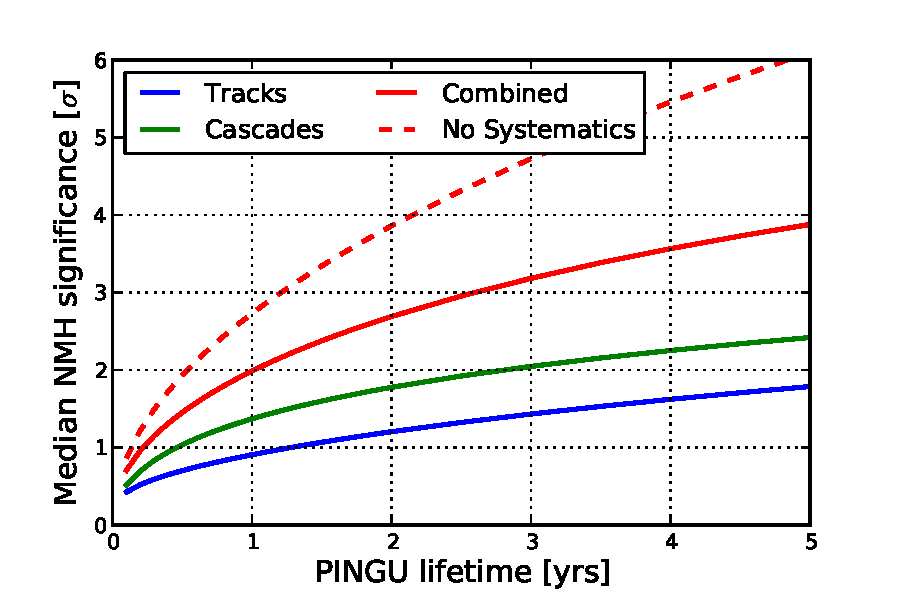
\includegraphics[width=0.495\linewidth]{sigma_vs_t_PIDV15_twochannel}}
 \subfloat[\label{fig:sigma_vs_t_threechannel}]
  {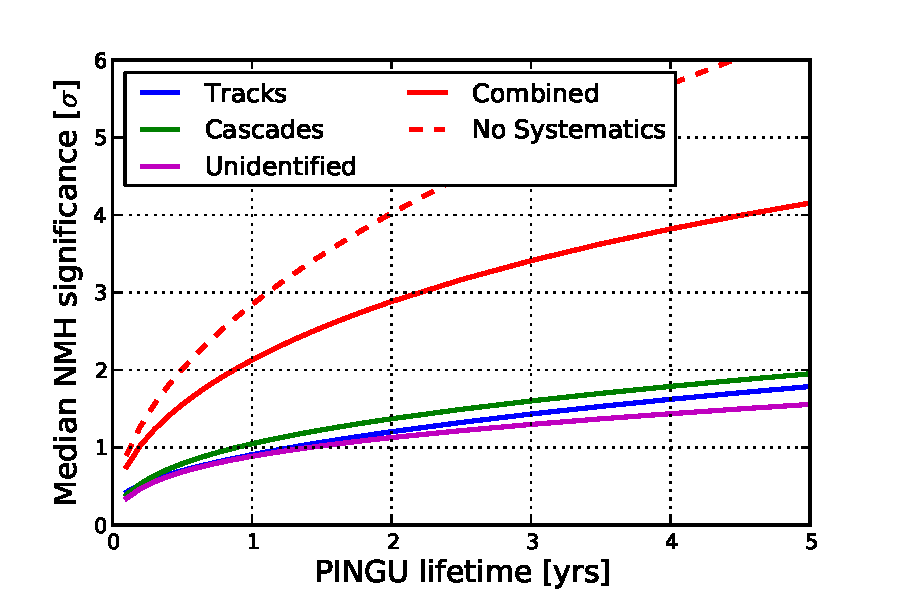
\includegraphics[width=0.495\linewidth]{sigma_vs_t_PIDV15_threechannel}}
 \caption{Individual and combined mass hierarchy sensitivity for the
   baseline model with V15 particle identification with two (a) and three
   (b) channels.}
 \label{fig:sigma_vs_t_HQPID}
\end{figure}

\noindent
Thus far, the particle identification has been considered as a binary decision,
classifying each event as either track-like or cascade-like, based on a BDT 
score (cf.\ Sec.~\ref{sec:cuts_PID}). Yet \papa offers the option to have 
separate event selections for tracks and cascades, such that \eg the cascade 
channel is populated only by events that actually ``look like cascades'' rather 
than events that just ``do not look like tracks''. To make sure that a given 
event does not end up in both samples, the decision should be based on the same 
BDT, but now with two cut values. Then the scores below the lower cut would 
then \eg correspond to cascades while the ones above the higher cut would be 
classified as tracks. All events with scores between the two cut values would 
end up in the ``unidentified'' sample.

Such an event selection does only exist for an anterior geometry version of 
PINGU, V15, that was used for intense systematic and reconstruction studies 
before optimising the geometry for maximal sensitivity to the mass hierarchy. 
The identification efficiencies are plotted in Fig.~\ref{fig:PID_threechannel}, 
with the corresponding function definitions listed in 
App.~\ref{app:PID_threechannel}. Note that the track identification efficiency 
is much better than for the baseline geometry V36, shown in Fig.~\ref{fig:PID}, 
since due to an error in the simulation configuration all Monte Carlo for V15 
was produced without generating noise hits on the PINGU optical modules, 
resulting in very clear event signatures.

The resulting significances are shown as a function of time in 
Fig.~\ref{fig:sigma_vs_t_HQPID}. As expected from the improved track
identification \wrt the baseline settings, already the two-channel significance
(Fig.~\ref{fig:sigma_vs_t_twochannel}) is enhanced compared to the baseline.
When opening the third channel of unidentified events
(Fig.~\ref{fig:sigma_vs_t_threechannel}), the cascade channel loses sensitivity
due to the reduced statistics and is now at approximately the same level as the
track channel, which remains unchanged. The unidentified events alone yield a
significance on the scale of tracks and cascades individually as well, yet they
suffer slightly stronger from systematic effects\footnote{This is apparent from
the fact that the curves for tracks and unidentified events lie on top of each
other for lifetimes below one year, but the track significance keeps to increase
stronger as more statistics gets accumulated.}. The full error listings are
tabulated in App.~\ref{app:fisher_threechannel}.

This behaviour is expected as the event selection for tracks stays the same as
in the two-channel settings while the cascade sample gets split into two
subsamples. Comparing the two corresponding error
listings---Tabs.~\ref{tab:fisher_PID_cscd_nontracks} for the case of all
``non-track'' events being combined into one channel as in the baseline model
and \ref{tab:fisher_PID_cscd_twochan} for having separate cascade and
unidentified channels and combining the respective Fisher matrices---the
statistical error on
the mass hierarchy parameter $h$ is slightly higher when the cascade channel is
split due to larger relative statistical errors. The systematic uncertainty on
$h$ on the other hand is reduced for the separate analysis, leading to the
expected overall increase in sensitivity. Yet this increase is rather moderate,
indicating that there is not much gain to be expected from moving further into
this direction\footnote{As an extreme, one could imagine to open a third axis
on the event histogram by introducing a Bj\"{o}rken-y-like variable, \eg the
ratio of cascade and track energy reconstructed by HybridReco/MultiNest.}.

For the remaining parameters one can see that \eg the impact of the
relative flux scaling $r_{\Phi,\,\nue-\numu}$ is reduced for the separated
analysis, driven by the high-purity cascade sample that has only a small
contamination of \numu events. Additionally, now the parameter $s_\mathrm{PID}$,
scaling the overall cascade and track identification efficiencies, comes into
play for the three-channel analysis, as it is no longer degenerate with the
overall normalisation $n_\aeff$ (at least for the unidentified channel), yet it
has no noticeable impact on the expected mass hierarchy significance.


\subsection{The Missing Monte Carlo Effect}
\label{sec:results_mcstats}

In Sec.~\ref{sec:sim_idea} it was pointed out that the ``conventional''
approach to evaluate PINGU's sensitivity to the neutrino mass hierarchy, \ie to
propagate the full Monte Carlo detector simulation through the analysis, is not
only computationally challenging, but introduces a bias towards too high
significances if the amount of available MC statistics is insufficient. This
effect can be demonstrated using an event reconstruction based on individual
Monte Carlo events processed for the earlier PINGU geometry V15.

\begin{figure}[thp]
 \centering
 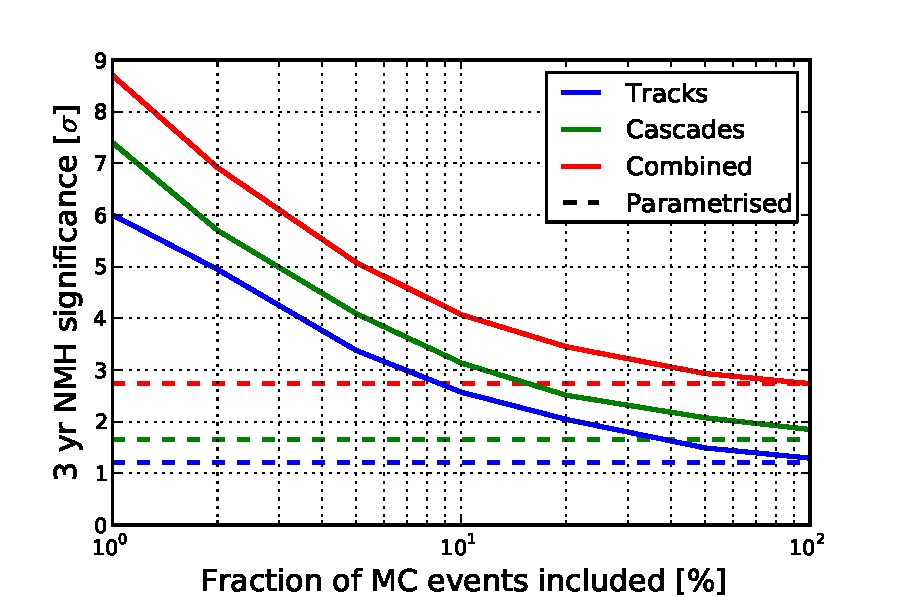
\includegraphics[width=0.7\linewidth]{sigma_vs_MCstat}
 \caption{PINGU's sensitivity to the neutrino mass hierarchy with
  reconstruction from MC data for geometry V15. The result for a reconstruction
  parametrisation from the same data is shown for reference.}
 \label{fig:sigma_vs_MCstat}
\end{figure}

For this geometry, enough MC events have been generated and
processed\footnote{For the most important channels, \nue and \numu,
$\approx 270,000$ and $\approx 340,000$ events are available, respectively. In
addition, $\approx 40,000$ \nutau and $\approx 80,000$ \nux NC events could be
used for this study.} to use them for the reconstruction in \papa directly. The
the reconstruction kernels were created by histogramming the MC events
as described in Sec.~\ref{sec:papa_code}, \ie now option (b) is used for
calculating the reconstructed histograms. This is repeated multiple times, 
reducing the fraction of the total number of events that is actually filled into
the kernels from 100\,\% to 1\,\%. Additionally, a reconstruction
parametrisation is fitted to the full dataset, which is given in
App.~\ref{app:reco_V15}.

In Fig.~\ref{fig:sigma_vs_MCstat}, the resulting mass hierarchy significances
for three years of PINGU lifetime are shown as a function of the fraction of MC
data used for the reconstruction. Only for the full amount of statistics a
relatively stable result is achieved, which is also consistent with the
parametrised reconstruction.

\begin{figure}[p]
 \centering
   Tracks \hspace{5cm} Cascades\\
   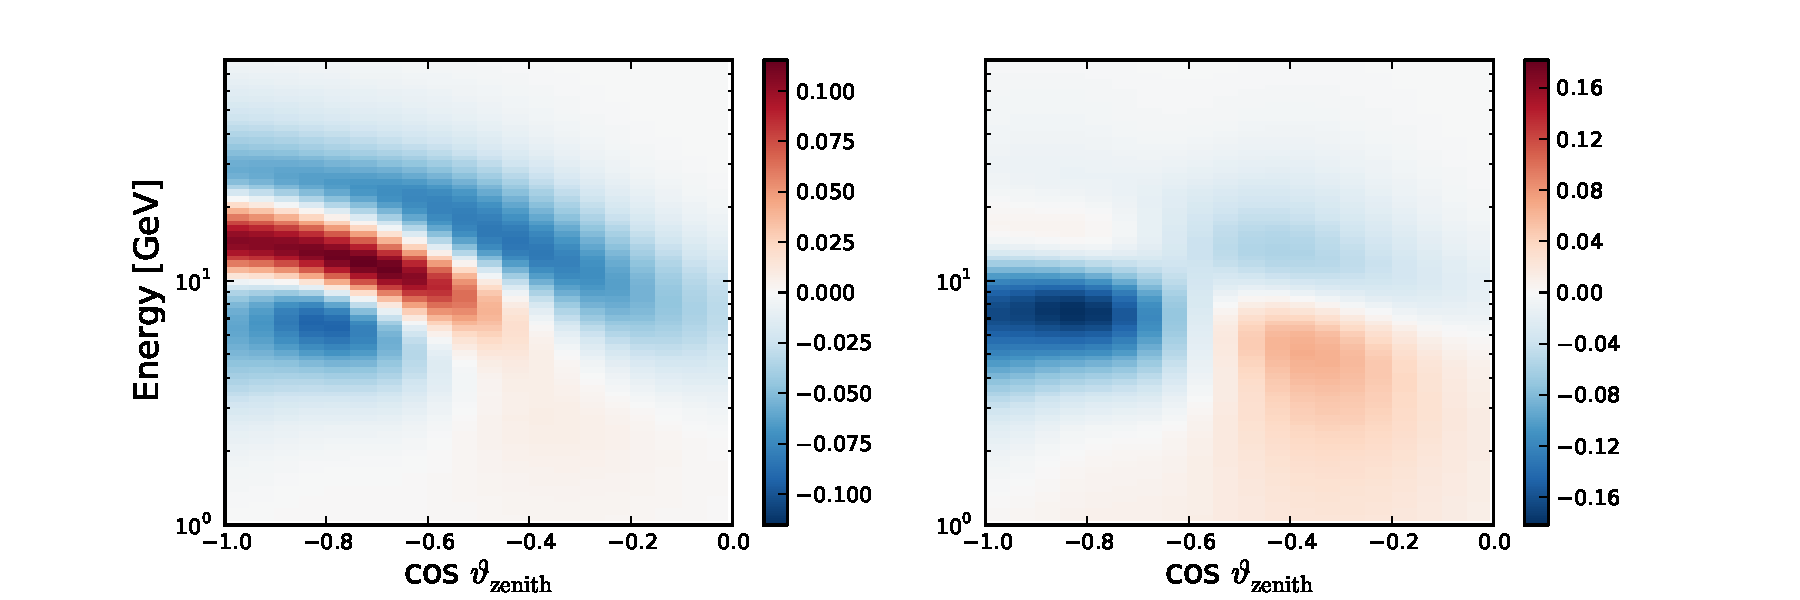
\includegraphics[width=\columnwidth]{Akhmedov_param_V15}
   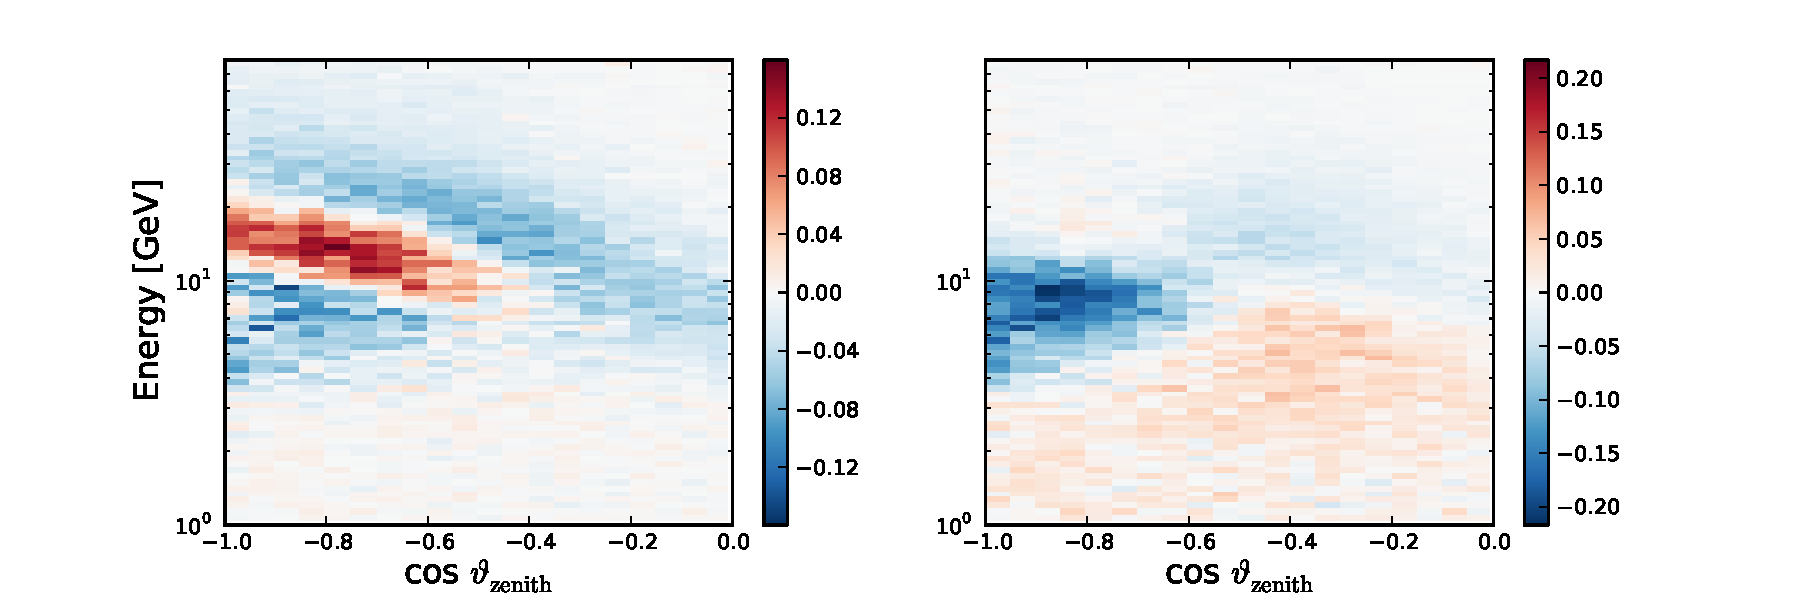
\includegraphics[width=\columnwidth]{Akhmedov_factor_1} 
   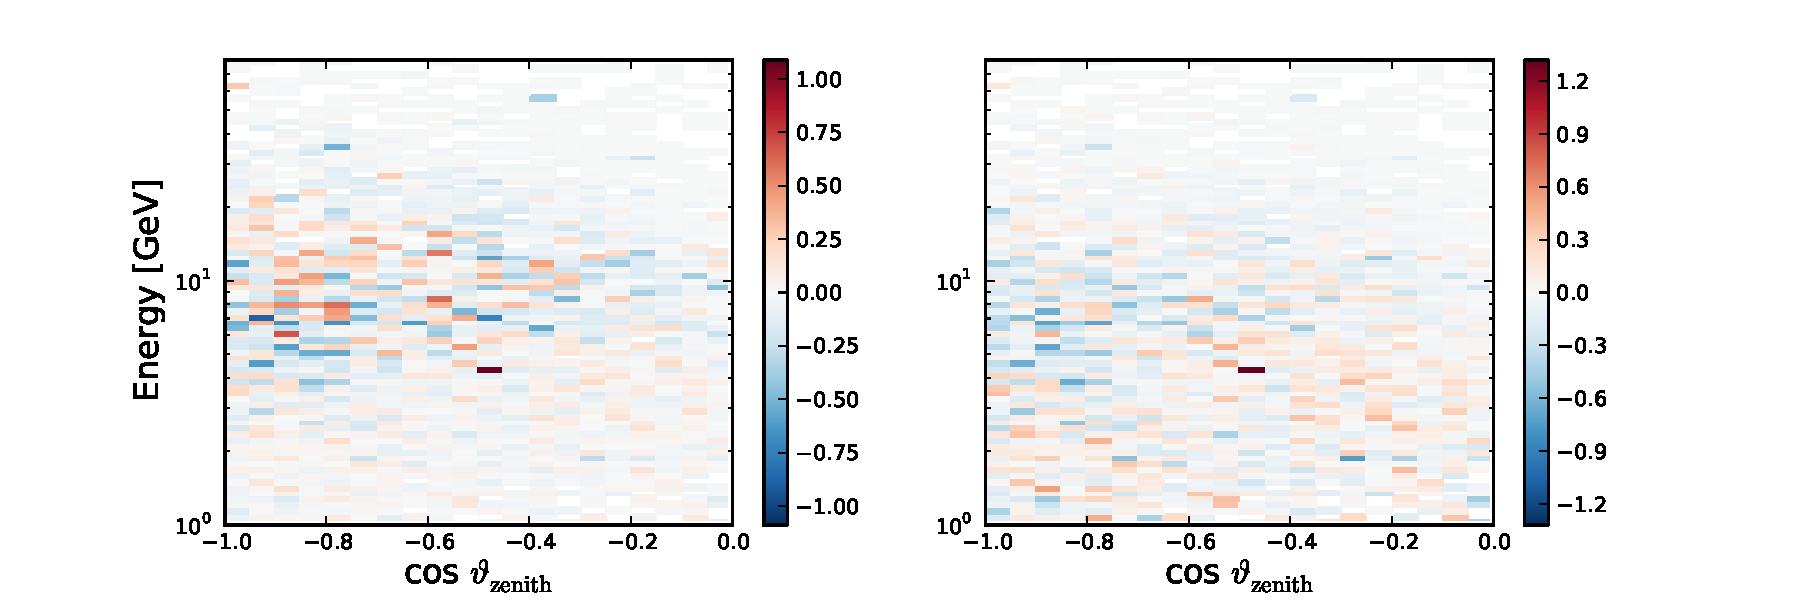
\includegraphics[width=\columnwidth]{Akhmedov_factor_100}
 \caption{\delchi distribution in the track (left) and cascade (right) channels
   for (top to bottom) the reconstruction parametrisation based on geometry V15
   and the reconstruction directly from 100\,\% and 1\,\% of the Monte Carlo
   events available for V15.}
 \label{fig:akhmedov_MCstats}
\end{figure}

The reason for this behaviour can be found when inspecting the \delchi
distributions for the different settings, shown in
Fig.~\ref{fig:akhmedov_MCstats}. When using the full sample of MC events
(middle panel), the pattern generated with the parametrised reconstruction is
reproduced quite accurately, reflected in the resulting significance values
being in agreement. For the extreme case of populating the reconstruction
kernels with only 1\,\% of the available events, the pattern imprinted by the
mass hierarchy difference has almost completely vanished and is replaced by
random fluctuations.

However the scale of the \delchi values is much higher in the histograms for
very low MC statistics, as one can see from the range of the colour scale,
which is linked to the highest individual bin value. 
The reason for this is that if the kernel tables are underpopulated, the 
reconstruction resolution effectively gets enhanced: When the statistics is 
sufficient, the hierarchy sensitivity of a single bin in the histogram of true 
energy and zenith angle is smeared out into the surrounding bins. If, in the 
extreme, only one MC event falls into this bin, its sensitivity is not smeared 
out, but only moved to a single other bin in the reconstructed histogram (the 
one where the single event is reconstructed in). The full sensitivity from 
the true histogram being retained at one point now increases the total 
significance as it is given by quadratically summing all individual 
bins.
% \footnote{As an illustration imagine a histogram with only two bins, where 
% the signal one is looking for is two events appearing in bin 1, however the 
% event reconstruction just randomly puts the appearing events into bin 1 or 2. 
% If the reconstruction is modelled properly, one would end up with one event in 
% each bin and a significance $\mathcal{S}=\sqrt{\sum 
% \left(n_i/\sqrt{n_i}\right)^2}=\sqrt{(1/\sqrt{1})^2 + 
% (1/\sqrt{1})^2}=\sqrt{2}$. If the two events are just moved to a random bin 
% together, the significance is $\mathcal{S}=\sqrt{0^2 + 
% (2/\sqrt{2})^2}=\sqrt{2}$} .

% Thus there are few
% individual bins that get weighted up dramatically by statistical fluctuations
% and hence artificially enhance the inherent significance of the whole
% histogram.

% That the bias introduced by these statistical fluctuations is 

